\chapter{Datasets, Topologies and Architecture comparison}

\section{Datasets}
CNN are trained on datasets. Each dataset consists of specific type of images and each of them are used in different tasks such as image classification or image captioning etc. The team has decided to use ImageNet as our primary dataset for the project.
\subsection{ImageNet}
It is one of the most prominent dataset used in the field of visual object recognition. In 2009 this dataset was first introduced to the world in the Conference on Computer Vision and Pattern Recognition by the computer science department of  Princeton University. It has over 14 million images and over 20000 categories. A large portion of the images has been hand annotated which can be helpful in the task of image captioning. Every year ImageNet runs a challenge called the ImageNet Large Scale Visual Recognition Challenge (ILSVRC), where different software architectures and algorithms take part in order to classify images of the dataset correctly. By 2017 most of the algorithms working on ImageNet have already achieved the accuracy of more than 95\%.


\subsection{ Reasons for Selection of ImageNet Dataset}
Reasons for selecting ImageNet are as follows:
\begin{itemize}
    \item The topologies that are going to be used in the project are well optimized for ImageNet. 
    \item On the other hand, ImageNet provides a greater challenge and also the topologies that are going to be used have already used ImageNet dataset. Hence their result can be used as a benchmarking performance for the implementation in the project.
\end{itemize}
\section{Topologies}
Here, we describe the CNN topologies that we will be deploying in our project. ResNet 50 and GoogLeNet are some of the state-of-the-art topologies that have performed exceptionally well on the ImageNet challenge. It is due to this reason we made the decision for their deployment so as to investigate how their performance can be improved through FPGA acceleration while maintaining the classification accuracy. The following sections give a detailed explanation about their architectures and basic working principles.

\subsection{GoogLeNet}\label{GoogLeNet_Topo}
GoogLeNet is a deep convolutional neural network and is also known as Inception-V1. It is also a winner of the ILSVRC 2014 in image classification. The architecture is based on the Hebbian principle which states that \textit{cells that fire together wire together} with the intuition of multi-scale processing. GoogLeNet is 22 layer deep network and used for object detection and classification. It has modules known as Inception which is a network within a network. GoogLeNet does not have any fully connected layers but uses global average pooling which keeps the model from overfitting the data. It was able to achieve a top-5 error rate of 6.67\% and requires only 4 million parameters, in comparison to this AlexNet requires up to 60 million parameters.

\begin{figure}[h!]
    \centering
    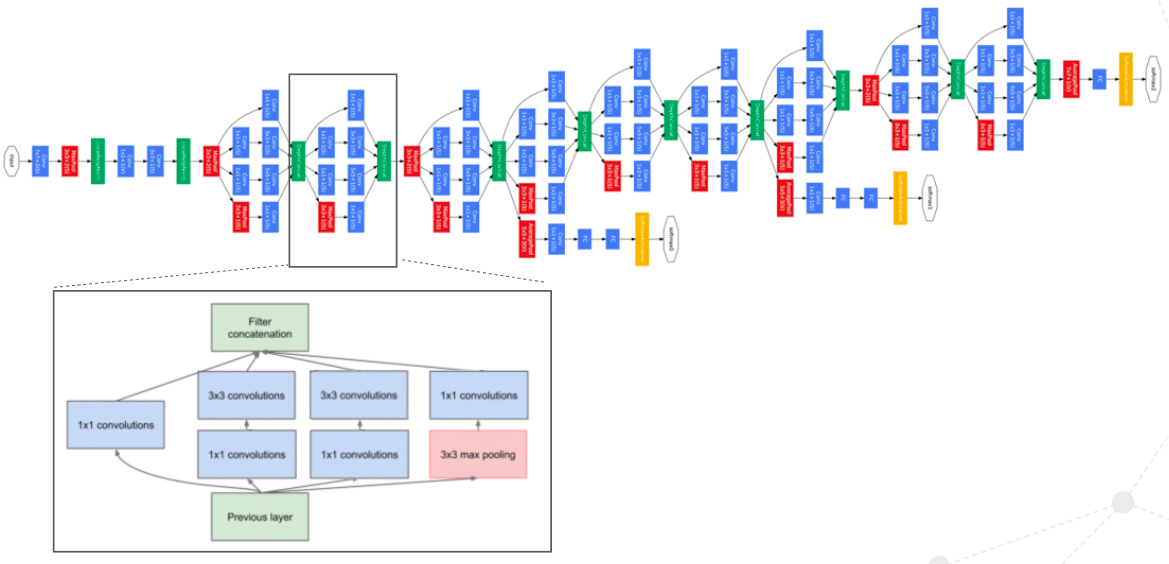
\includegraphics[scale=0.4]{img/googlenetarch.png}
    \caption{GoogleNet Architecture}
\end{figure}

\subsubsection{Inception Module}
The logic behind Inception architecture is built on finding optimal local sparse structure in the convolution network and to repeat it spatially. There are 9 inception modules in GoogLeNet. Each inception module has 6 convolution layers and 1 max pooling layer spread across 4 branches within the inception module. Some convolution layers and max pool layer are stacked on each other (branch 3) due to which four different outputs are created within the inception module which is concatenated to produce one single output. This output is then passed onto the next inception module and so forth. Concatenation of this output filter occurs based on depth. The 1x1 convolution layers in inception module help us to preserve spatial dimensions and to reduce the feature depth.

The output from the last inception module is forwarded to global average pooling.

\begin{figure}[h!]
    \centering
    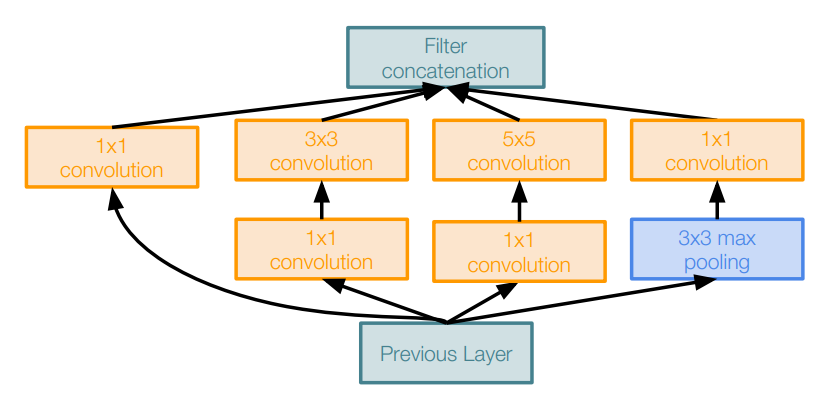
\includegraphics[scale=0.4]{googlenet}
    \caption{Inception Module}
\end{figure}

\subsection{ResNet 50}
ResNet is a deep neural network released by Microsoft and, also a winner of the ILSVRC 2015 in image classification, detection, and localization. ResNet is a series of DNN with different number of layers from 18 to 152. Here we are implementing the ResNet neural network with 50 layers.
\newline
The ResNet 50 architecture is divided into 4 blocks. These 4 blocks comprise of 16 units. The units in the blocks are combined based on the depth, i.e, all the units in the block have the same depth. The units of the ResNet 50 consist of 2 1 $\times$ 1 convolution kernels and 1 3 $\times$ 3 convolution kernel. Similar to concat layer in GoogleNet, here we have Eltwise layer which performs element wise addition and generates the output. This ouptut is then fed as an input to the next unit. ResNet uses an special type of connections called as skip connection.  

\begin{figure}[h!]
\centering
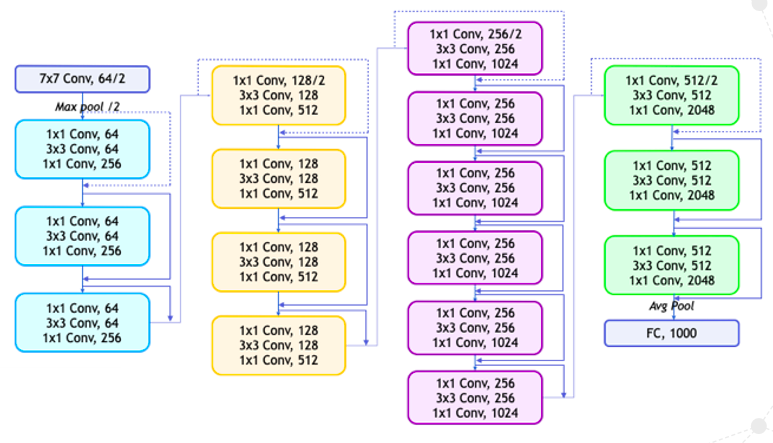
\includegraphics[scale=0.5]{img/Resne50arch.png}
\caption{ResNet 50}
\label{fig:resnet_50}
\end{figure}

\subsubsection{Skip Connections}
The base idea is applying the residual connections which are described as learning the residual representation of functions instead of signal representation. One of the conceptual ideas of ResNet is using the skip connection. Skip connection makes the network deeper.

Many convolution DNNs run into a problem with vanishing or exploding gradients because, during backpropagation, we derive error function with respect to the current weight and get multiplying of small or large numbers. The product of small numbers will be zero (vanished) and the product of large numbers will be too large (exploded). Developers of ResNet solved this problem by using a skip connection. In the skip connections for the next layer, they use the input from the previous layer without any modification. 

The output of skip connection is  F(x) + x and the weight layers actually are to learn a kind of residual mapping: output minus identity x. If we have a vanishing gradient we always have an identity x to send it back to previous layers. 

After each convolution layer, ResNet uses the batch normalization from Inception-v2. 

\begin{figure}[h!]
    \centering
    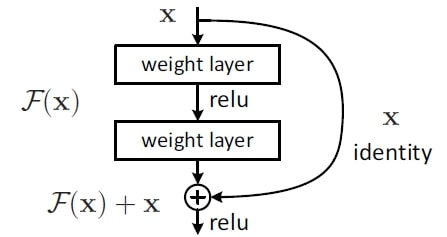
\includegraphics[scale=0.4]{resnet_1}
    \caption{Skip connection}
\end{figure}

The main concepts of constructing ResNet:
\begin{itemize}
\item Avoiding representational bottlenecks by not abruptly reducing the dimension of data, but smoothly from the beginning of the network to the classifier at the output.
\item Factorization of convolution layer into smaller pieces because this will save resources and help to increase the count of layers.
\item Supporting a balance between the depth and width of the network. You should increase or decrease both dimensions.
\end{itemize}

Figure \ref{fig:resnet_50} shows the whole scheme for ResNet 50.

